\documentclass{book}
\usepackage[subpreambles=false]{standalone}

%%%%%%%%%%%%%%%%%%%%%%%%%%%
% Silence warning messages
\usepackage{silence}
\WarningsOff[scrlayer-notecolumn]
\WarningsOff[biblatex]

%%%%%%%%%%%%%%%%%%%%
% Commenting

%\usepackage[author=Lyndon]{pdfcomment}
%\newcommand{\pdfcomment}[1]{} %ignore all comments

%\usepackage{todonotes}
%\newcommand{\pdfcomment}{\todo}


%%%%%%%%%%%%%%%%%%%%
% Tables
\usepackage{booktabs}

%%%%%%%%%%%%%%%%%%%
% Fonts
\usepackage{tgadventor} %sans
\usepackage{tgpagella}  %serif
\usepackage{inconsolata} %mono
\usepackage[T1]{fontenc}

\usepackage{microtype}
\usepackage[all]{nowidow}
%%%%%%%%%%%%%%%%%%%%%%%
% Styling
\setcounter{secnumdepth}{4}
\setcounter{tocdepth}{2}

\usepackage{placeins}



%%%%%%%%%%%%%%%%%%%
% Math
\usepackage{amsmath, amssymb, stmaryrd, mathtools}
\DeclareMathOperator*{\argmin}{argmin}
\DeclareMathOperator*{\argmax}{argmax}

\usepackage{xparse,xstring,etoolbox}
% crossref this against notation section
\newcommand{\vv}[1]{\tilde{#1}} % vector
\newcommand{\seq}[1]{\mathcal{#1}} % sequence
\newcommand{\set}[1]{\mathbb{#1}} % set

%%%%%%%%%
% Indexing/sequence indexing
\newcommand{\seqind}[2]{#1^{#2}} % seqence index
\newcommand{\ind}[2]{#1_{#2}} % indexed
\newcommand{\disamb}[2]{#1^{\mathrm{#2}}} %disambiguated

%% Smart indexing and naming
\newcommand{\ifupper}[3]{
    \normalexpandarg
	\exploregroups
	\StrCount{ABCDEFGHIJKLMNOPQRSTUVWXYZ}{#1}[\uppercount]
	\ifnumgreater{\uppercount}{0}{#2}{#3}
}

%smart index
\DeclareDocumentCommand{\ii}{u{_} m}{
	\ifupper{#1}%
	{% just a single uppercase character, i.e. a matrix
		  %make sure the index is the right length
		\StrCount{#2}{,}[\indcount]
		\ifnumgreater{\indcount}{0}
		{ % Got multiple indexes so all good
		 	\ind{#1}{#2}
		}
		{ % Only 1 index so grab the column
		 	\ind{#1}{{:,#2}}
		}
	}%
	{% Not just a single upper case character
		\ind{#1}{#2}
	}
}

\DeclareDocumentCommand{\nn}{u{_} m}{
	\seqind{#1}{#2}
}

\DeclareDocumentCommand{\dd}{u{_} m}{
	\disamb{#1}{#2}
}

% Index of a vector
\DeclareDocumentCommand{\iv}{u{_} m}{\ii{\vv #1}_{#2}}
\DeclareDocumentCommand{\dv}{u{_} m}{\dd{\vv #1}_{#2}}
\DeclareDocumentCommand{\nv}{u{_} m}{\nn{\vv #1}_{#2}}

%exp
\let\oldexp\exp
\renewcommand{\exp}[1]{\oldexp \left( #1 \right)}
\newcommand{\exptwo}[1]{\oldexp_2 \left( #1 \right)}

\newcommand{\softmax}{\mathrm{smax}}

\DeclareMathOperator*{\expectedop}{\mathbb{E}}
\DeclareDocumentCommand{\expected}{u{_} m}{
	\expectedop\limits_{\mathrlap{#2}}
}

%%%%%%%%%%%%%%%%
%Graphics
\usepackage{tikz}
\usetikzlibrary{positioning, fit,  shapes.geometric}
\usepackage{ifthen}
\usepackage{etoolbox}

\tikzset{
	backgroundcolor/.style ={fill=white},
	every node/.append style={
		minimum height=7mm,
	},
	labe/.append style={
		%Blue,
		align = center,
		backgroundcolor,
		fill opacity=0.6,
		text opacity=1,
		font={\footnotesize\itshape}	
	},
	layer/.append style={
		draw,
		align = center,
		minimum height=7mm,
	},
	tight/.append style={
		inner sep=0.2mm,
	},
	lookupbox/.append style={
		draw=none,
		append after command={
		       	[shorten <= -0.5\pgflinewidth]
		       	([shift={(-1.5\pgflinewidth,-0.5\pgflinewidth)}]\tikzlastnode.north east)
		       	edge([shift={( 0.5\pgflinewidth,-0.5\pgflinewidth)}]\tikzlastnode.north west) 
		       	([shift={( 0.5\pgflinewidth,-0.5\pgflinewidth)}]\tikzlastnode.north west)
		       	edge([shift={( 0.5\pgflinewidth,-1.5\pgflinewidth)}]\tikzlastnode.south west)            
		       	([shift={( -1.5\pgflinewidth,+0.5\pgflinewidth)}]\tikzlastnode.south east)
		       	edge([shift={(-1.5\pgflinewidth,-0.5\pgflinewidth)}]\tikzlastnode.north east)
		},
		inner sep=0.7mm,
		outer sep=0mm,
		minimum width=25mm
	}
}

\usepackage{pgfplots}
\pgfplotsset{compat=1.14}
\pgfplotsset{sideplot/.append style={
		width=\notescolwidth,
		domain=-10:10,
		samples=101,
		smooth,
		enlarge y limits={abs=2},
		axis lines=middle,
		xlabel  = $z$,
		ylabel  = $y$,
	},
	equ/.append style={
		color=blue,
		thick,
		mark=none
	}
}

% Function  For a plot 
% it  needs to be declared in preamble because of how \makenote* interacts with multiple files
\def\errorsurface(#1,#2){(0.5*#1 + 0.7*#2 + sin(deg(1.5*#1 + #2^2)))^2}


\usepackage{graphicx}
\graphicspath{{./figs/}, {./}, {./figs/chaptersentencerrepr/}, {./figs/chapterintromachinelearning/}, {./figs/chapterwordrepr/}}
\usepackage{adjustbox}


%%%%%%%%%%%%%%%%%%%
% Refs
\usepackage{cleveref}

\addbibresource{master.bib}

%%%%%%%%%%%%%%%%%%%%
% Formatting

% for examples from natural language space.
\newcommand{\natlang}[1]{\ifmmode \text{``\texttt{#1}''} \else {``\texttt{#1}''}\fi}
% \ifmmode ``trick'' from https://tex.stackexchange.com/a/15194/5834

%%%%%%%%%%%%%%%%%%%%%



\begin{document}
\bookmarksetup{startatroot}
\addtocontents{toc}{\protect\vspace{12pt}}
\chapter{Conclusion}
Current research in natural language understanding relies on 
the creation of representations of natural language that can be readily manipulated by computer algorithms
for purposes of making inferences about meaning.
This thesis has focused on one particular type of representation:
linear combinations of embeddings.
This is a very simple representation, closely related to a bag of words.
There is a machine learning adage: that given enough data and a model with sufficiently high representational capacity any problem can be solved.
However, we seem to have found a sweet spot, 
where a model seemingly without sufficiently high representational capacity,
never-the-less performs excellently on tasks with the amount of data that we have.
It seems clear that there will always exist low-medium resource settings where linear combinations of embeddings will remain an ideal method for many practical problems.


The research presented here on linear combinations of embeddings has shown that this simple input representation technique is surprisingly powerful.
This  power is related to the fact that surface level information plays a significant role in practically giving human understandable meaning to a natural language utterance.
Word content is the most obvious surface level information, and is effectively captured by a LCOWE.
The LCOWE represented this in a dense, but informative vector.
While the LCOWE loses word order information, it preserves the aggregated content very well,
making it very useful for the tasks considered in this research.


We considered a number of tasks to identify the utility of this representation.
\Cref{SentVecMeaning} investigated classifying paraphrases as a means to investigate the quality of SOWE as a sentence embedding method.
\Cref{ColorEst} defined models for color estimation from short phrases.
\Cref{RefittingSenses} considered if we could use weighted combinations of sense embeddings to better capture the sense used in a particular example.
\Cref{NovelPerspective} considered taking the mean of the embeddings adjacent to named entity tokens across a fictional text as a feature to characterize how the named entity token was being used.
We followed up these practical demonstrations of capacity,
with further investigations into what can be recovered from the SOWE in the important area of sentence representations.
\Cref{BOWgen} demonstrated a method that could partially recover bags of words from a given SOWE.
\Cref{SOWE2Sent} extended this work by attempting to order those bags of words into sentences.
This demonstrated that a surprising amount of information is still available in the summed embeddings; which helps to explain why they work so well.



Linear combinations of embedding are not perfect for representing all meaning,
as they do not encode any information about word order.
It is thus clear that there exists sentences and phrases that are ambiguous when represented this way.
However, we note that such sentences are rare: often there is only one likely ordering, particularly in any given text with a restricted domain.
Most sentences are relatively short; multiple similarly likely word ordering occur more often in longer sentences.
Many reorderings are paraphrases, or near paraphrases, particularly when done at the clause level.
Though some orderings, such as noun swaps of nouns with similar ontological classification (e.g. Agents, Objects) do exist at almost all lengths:
many are paraphrases \natlang{The banana is next to the orange} \emph{vs.} \natlang{The orange is next to the banana};
and others are similar in meaning: \natlang{The banana is to the left of the orange} \emph{vs.} \natlang{The orange is to the left of the banana}.
It is desirable that such sentences are nearby in a representational of the semantic space.


\section{Future work}

\subsection{Adversarial Test cases}
A limitation of the LCOWE representations is that they have no ability to represent word order.
This is in-contrast to RNNs and other commonly used neural network based representations of multi-word natural language input.
It is possibly to construct adversarial test cases, that no LCOWE can succeed on.
This can be done by selecting sentences with multiple reasonable word orders with very different meanings.
It is worth consideration,
that such adversarial test cases allow advancement of the state of the art to increase the capacity of models to represent all possible inputs.
However, they do not necessarily advance the practical state of the art in representing real inputs that occur in a particular domain. 
Thus it is  is essential to understand how common such adversarial test cases are in practice.

Future work in this area requires not just the construction of adversarial examples; but of the determination of how common they are in practice.
Adversarial examples are not ubiquitous in real world tasks.
It is important not to succeed on only these cases, while failing on the more common simple cases.

It is also important to consider how challenging an adversarial test case is.
In \Cref{ColorEst}, the ordered task which was to make predictions for colors for which the different words in the name could appear in different orders to describe different colors.
For example \natlang{bluish green} and \natlang{greenish blue} are different colors.
However, they are very \emph{similar} colors.
As such the error from discarding word order, is less than the error from using a more complicated model such as an RNN.
Such a more complex model is harder to train, and those practical difficulties can dominate over a small amount of theoretical lack of capacity.



\subsection{Language Models and Orderless Representations}


\begin{figure}
	\resizebox{\textwidth}{!}{
		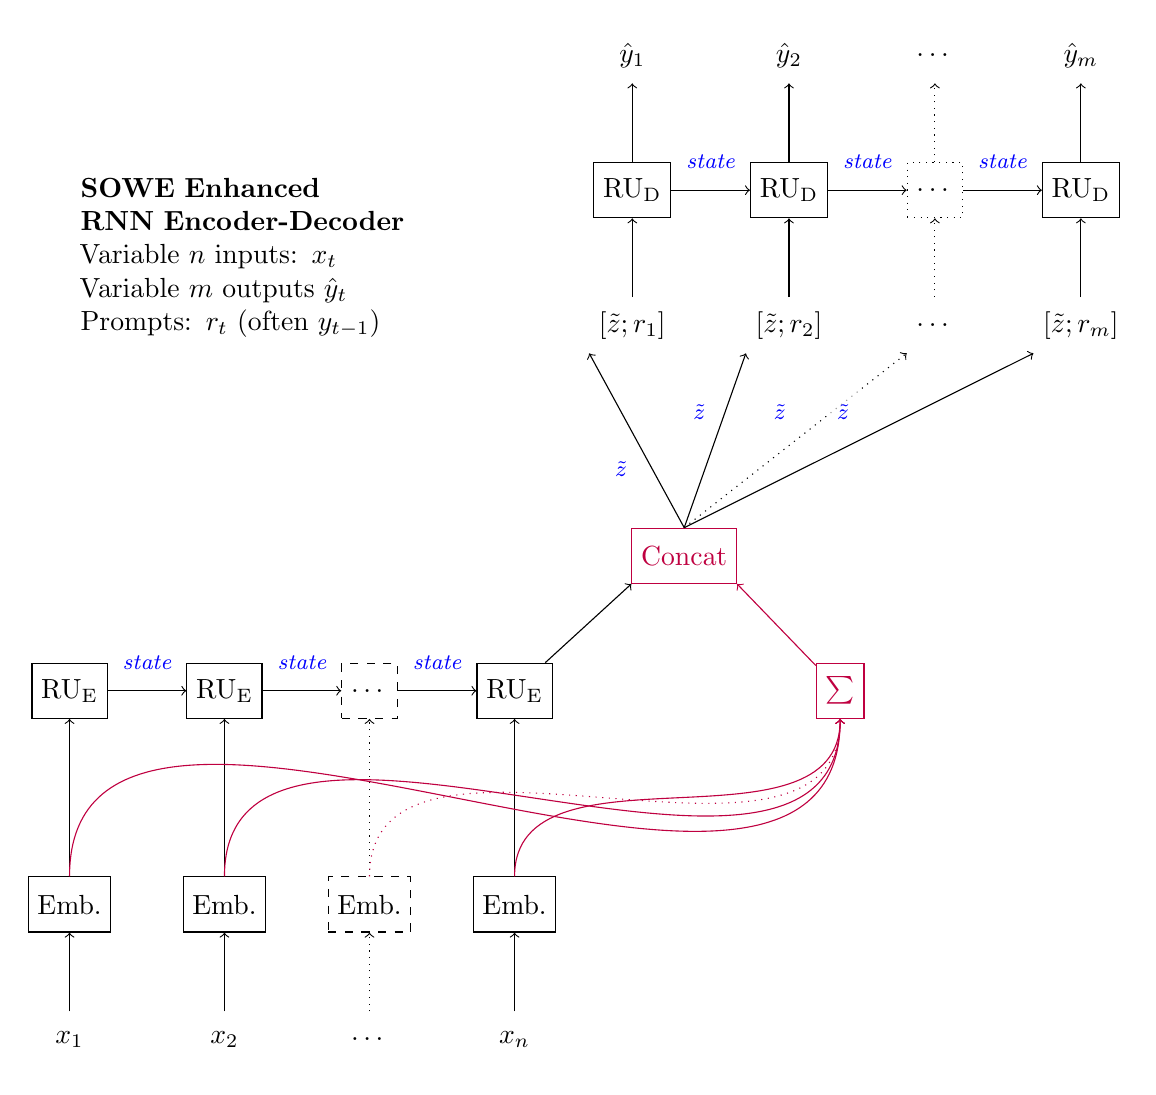
\begin{tikzpicture}[
		neo/.append style={purple},
		labe/.append style={
			auto,
			blue,
			align = center,
			backgroundcolor,
			fill opacity=0.6,
			text opacity=1,
			font={\footnotesize\itshape}	
		},
		layer/.append style={
			draw,
			align = center,
			minimum height=7mm,
		}
		]
		\numdef{\N}{8}
		\numdef{\labelwidth}{5.5cm}
		
		\node(lbl)[text width= \labelwidth] {\textbf{SOWE Enhanced\\RNN Encoder-Decoder}\\%
			Variable $n$ inputs: $\nv x_t$\\%
			Variable $m$ outputs $\nn \hat{y}_t$\\%
			Prompts: $\nv r_t$ (often $y_{t-1}$)
		};
		
		\coordinate[yshift = -5.5cm, xshift=-1.5cm] (L0) at (lbl.west);
		\numdef{\NN}{4}
		\foreach \I[count=\j from 0] in {1,...,\NN}{
			\ifnumequal{\I}{\NN - 1}{%
				\node(L\I)[dashed, layer, right = of L\j] {\ldots};
				\node(E\I)[layer, dashed, below = 2  of L\I]{Emb.};
				\node(w\I)[below = of E\I]{\ldots};
				\draw[->,dotted] (w\I) -- (E\I);
				\draw[->,dotted] (E\I) -- (L\I);
			}%
			{
				\node(L\I)[layer, right = of L\j] {$\mathrm{RU_E}$};
				\node(E\I)[layer, below = 2 of L\I]{Emb.};
				\node(w\I)[below = of E\I]{\ifnumequal{\I}{\NN}{$\nv x_n$}{$\nv x_\I$}};
				\draw[->] (w\I) -- (E\I);
				\draw[->] (E\I) -- (L\I);
			}
		}
		\foreach \I[count=\j from 1] in {2,...,\NN} {
			\draw[->] (L\j) edge node[labe] {state} (L\I);
		}
		
		
		
		\node (shared) [neo,  layer, above right = of L\NN]{Concat};
		\draw[->] (L\NN) -- (shared.south west);
		
		\node (sowe) [neo, layer, below right = of shared]{$\sum$};
		\draw[->, neo] (sowe) -- (shared.south east);
		\foreach \I in {1,...,\NN}{
			\ifnumequal{\I}{\NN - 1}{%
				\draw[neo, ->, dotted] (E\I.north) to[out=90,in=-90] (sowe.south);
			}%
			{
				\draw[neo, ->] (E\I.north) to[out=90,in=-90] (sowe.south);
			}
		}
		
		\coordinate[above = 6 of L\NN] (Lp\NN);
		\numdef{\NP}{\N - 1}
		\foreach \j in {\NN,...,\NP}{
			\numdef{\I}{\j+1}
			\numdef{\y}{\I - \NN}
			\ifnumequal{\I}{\N-1}{%
				\node(Lp\I)[dotted, layer, right = of Lp\j] {\ldots};
				\node(w\I)[below = of Lp\I]{\ldots};
				\node(y\I)[above = of Lp\I]{\ldots};
				\draw[->,dotted] (w\I) -- (Lp\I);
				\draw[->,dotted] (Lp\I) -- (y\I);
				\path[->,dotted] (shared.north) edge node[labe]{$\vv z$} (w\I.south west);
			}%
			{
				\node(Lp\I)[layer, right = of Lp\j] {$\mathrm{RU_D}$};
				\ifnumequal{\I}{\N}{
					\node(w\I)[below = of Lp\I]{$[\vv z; \nv r_m]$};
					\node(y\I)[above = of Lp\I]{$\nn \hat{y}_m$};
				}
				{
					\node(w\I)[below = of Lp\I]{$[\vv z; \nv r_\y]$};
					\node(y\I)[above = of Lp\I]{$\nn \hat{y}_\y$};
				}
				
				\draw[->] (w\I) -- (Lp\I);
				\draw[->] (Lp\I) -- (y\I);
				\path[->] (shared.north) edge node[labe]{$\vv z$} (w\I.south west);
			}
		}
		
		
		
		
		\numdef{\NNp1}{\NN + 1}
		\foreach \I in {\NNp1,...,\NP} {
			\numdef{\j}{\I+1}
			\draw[->] (Lp\I) edge node[labe] {state} (Lp\j);
		}
		\end{tikzpicture}
	}
	\caption{An encoder-decoder model with a SOWE encoder bypass layer added (shown in red). \label{fig:enhancedencoderdecoder}}
\end{figure}


There is a complementary aspect to LCOWE and language models.
While LCOWE have no capacity to handle word order, but they have an excellent ability to capture word content;
whereas pure language models have no ability to capture word content, but have an excellent ability to capture word order.
Language modelling based models incorporating a representation stage, such as encoder-decoders \citep{cho-EtAl:2014:EMNLP2014}, do not capture word content as well as LCOWE \citep{ac2018probingsentencevectors}.
They do, however, have state of the art order representation.

An interesting combination of the two,
would be an encoder model,
where the coding layer,
is augmented by concatenating the final RNN output, with a sum of word embeddings, for all the input words to the encoder.
An example of this for a encoder-decoder is shown in \Cref{fig:enhancedencoderdecoder}.
This would effectively allow a bypass of the encoder RNN.
A similar bypass of intermediate layers has been used in feed-forward networks including the notable neural probabilistic language model \citep{NPLM}.
The significant advantage of bypassing the RNN encoder is that it allows the model to weight the value of the orderful representation of the RNN output, against the unordered representation of the SOWE and learn use which ever is better for the task.
Further, having explicit access to the surface level features in the SOWE,
should help encourage the orderful encoder to learn more important deeper features.

A coding layer featuring components from a encoder capturing order-features, and a SOWE capturing surface features can be expected to perform better at both representations than either alone.
This expectation is due to the the weighting  above  the shared layer will train to weight each feature for what it is better at, and thus during gradient decent the weights for the encoder would be decreased for surface information that is better obtained from the SOWE.
It would thus allow each part of the network to \emph{focus} on what it is best at, thus  creating better representations./
This thesis has shown that SOWE can excel at surface level tasks (and that more tasks that expected are surface level).
On deeper tasks where structure becomes more important ordered representations out perform it \parencite{ac2018probingsentencevectors}.
By combining the two we expect to get the best of both worlds,
and produce truly excellent models for natural language understanding.




\end{document}